%%%%%%%%%%%%%%%%%%%%%%%%%%%%%%%%%%%%%%%%%%%%%%%%%%%%%%%%%%%%%%%%%
%%% %
%%% % weiiszablon.tex
%%% % The Faculty of Electrical and Computer Engineering
%%% % Rzeszow University Of Technology diploma thesis Template
%%% % Szablon pracy dyplomowej Wydziału Elektrotechniki 
%%% % i Informatyki PRz
%%% % June, 2015
%%%%%%%%%%%%%%%%%%%%%%%%%%%%%%%%%%%%%%%%%%%%%%%%%%%%%%%%%%%%%%%%%

\documentclass[12pt,twoside]{article}
\usepackage[hidelinks]{hyperref}
\usepackage{weiiszablon}
\usepackage{float}

\author{Beniamin Motyka}

% np. EF-123456, EN-654321, ...
\studentID{EF-160780}

\title{Interaktywny system e-learningowy o zagrożeniach w obszarze cyberbezpieczeństwa}
\titleEN{Temat pracy po angielsku}


%%% wybierz rodzaj pracy wpisując jeden z poniższych numerów: ...
% 1 = inżynierska	% BSc
% 2 = magisterska	% MSc
% 3 = doktorska		% PhD
%%% na miejsce zera w linijce poniżej
\newcommand{\rodzajPracyNo}{1}


%%% promotor
\supervisor{dr Michał Piętal}
%% przykład: dr hab. inż. Józef Nowak, prof. PRz

%%% promotor ze stopniami naukowymi po angielsku
\supervisorEN{(academic degree) Imię i nazwisko opiekuna}

\abstract{Treść streszczenia po polsku}
\abstractEN{Treść streszczenia po angielsku}

\begin{document}

% strona tytułowa
\maketitle

\blankpage

% spis treści
\tableofcontents

\clearpage
\blankpage

\clearpage
\section{Wprowadzenie}

W dzisiejszych czasach śmiało można stwierdzić, iż	internet jest istotną częścią codzienności każdego z nas. Ostatnimi laty, stał się on jeszcze bardziej bliskim i niezbędnym narzędziem dla wielu, za sprawą pandemii COVID-19 - sprawiła ona bowiem, że pewne dziedziny życia, takie jak dydaktyka czy praca wykonywana umysłowo, przeszły swoistą transformację. Miejsca, w których spotykali się studenci wraz z wykładowcami, czy pracownicy w biurze, stały się puste. Zastąpiła je komunikacja zdalna -- przez internet. Pandemia spowodowała również, że znacząco zmienił się profil przeciętnego użytkownika Internetu.

Fakt, iż ludzkość została zmuszona, by przenieść znaczną część swojego funkcjonowania do sieci internet, niesie ze sobą poważne konsekwencje. Szybkie jak do tej pory tempo rozwijania się technologii informatycznych stało się nieporównywalnie bardziej dynamiczne, a co się z tym wiąże, obecne w sieci liczne zagrożenia stały się coraz powszechniejsze i trudniejsze w identyfikacji. 

\subsection{Cel i zakres pracy}

Celem niniejszej pracy inżynierskiej jest wyeksponowanie, opis oraz implementacja najbardziej pospolitych zagrożeń i luk bezpieczeństwa w Internecie nie tylko z perspektywy zwykłych użytkowników, ale również dla małych i średnich przedsiębiorstw (MMŚP). Na podstawie wiedzy wyniesionej ze studiów stworzona została aplikacja internetowa, zwierająca interaktywne kursy o tematyce cyberbezpieczeństwa z elementami wirtualnej rzeczywistości oraz quizami, podsumowującymi wiedzę kursanta po kursie. Każdy kurs podzielić można na podstawowy, zawierający zasadnicze informacje na określony temat i zaawansowany, dla kursantów chcących bardziej zgłębić wybrany obszar. Kurs kończy się quizem jednokrotnego wyboru, na którego końcu zostaje przedstawiony wynik zdającego wraz z prawidłowymi odpowiedziami. Ma on na celu zweryfikowanie i ustrukturyzowanie wiedzy użytkownika po ukończonym szkoleniu. Celem zapewnienia większej dostępności szerszemu gronu odbiorców, aplikacja, wraz z treścią kursów, została w całości przetłumaczona na język angielski.

Treść prezentowana podczas kursów wykorzystuje elementy wirtualnej rzeczywistości (VR) w podstawowym stopniu. Kursy pozwalają użytkownikom symulować sytuacje zagrożeń bezpieczeństwa na wirtualnym komputerze czy telefonie. Nie tylko polepsza to końcowe odczucia kursanta, poprzez dostarczenie mu bardziej jakościowej treści, ale także bezpośrednio wpływa na jakość przyswajanej wiedzy. Zostało bowiem udowodnione, że doświadczanie sytuacji zbliżonych do rzeczywistości poprzez interakcję i immersję polepsza proces uczenia się. \cite{VrLearning}

Dzięki temu, że powyższa idea została zrealizowana w formie aplikacji klasy e-learning wraz z elementami wirtualnej rzeczywistości, istnieje realna szansa na zwiększenie świadomości społecznej, edukację oraz poprawę zabezpieczeń systemów teleinformatycznych i infrastruktury sieciowej. W zakres pracy wlicza się takie zagadnienia jak:
\begin{itemize}
\item Przegląd, dokumentacja i implementacja zagrożeń i luk bezpieczeństwa w sieci. 
\item Przygotowanie i wyselekcjonowanie najważniejszych elementów dla kursantów.
\item Stworzenie aplikacji e-learningowej przy użyciu technologii opisanych w kolejnym rozdziale. Użytkownicy będą mogli wziąć udział w interaktywnej prezentacji każdego z zagrożeń, wraz z weryfikacją efektów kształcenia.
\item Zasugerowanie potencjalnych rozwiązań w odniesieniu do opisanych cyberzagrożeń.
\item Przedstawienie wniosków płynących z powyższych oraz dalszych planów na rozwój projektu.\\
\end{itemize} 

\clearpage

\section{Technologie wykorzystane w aplikacji}

Projekt opisany w niniejszej pracy inżynierskiej składa się z dwóch aplikacji. Pierwsza z nich -- aplikacja działająca po stronie klienta -- została wykonana z użyciem biblioteki React. Jej głównym przeznaczeniem jest warstwa graficzna (tzw. UX, ang. User Experience), z którą użytkownik wchodzi w interakcję. Jest odpowiedzialna za dynamikę strony i wyświetlane na niej treści. Przesyła również informacje od użytkownika do drugiej aplikacji -- API -- która działa stronie serwera i komunikuje się z nierelacyjną bazą danych MongoDB. Opisane API zostało wykonane w technologii GraphQL, w oparciu o środowisko uruchomieniowe Node.js i bibliotekę Express. Architekturę systemu można przedstawić następującym diagramem:

\begin{figure}[H]
	\centering
	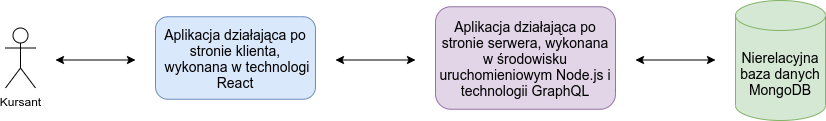
\includegraphics[width=1\linewidth]{figures/app-architecture}
	\caption{Architektura systemu}
	\label{fig:system-architecture}
\end{figure}

\subsection{JavaScript}

JavaScript to skryptowy język programowania powstały w latach 90. ubiegłego wieku, umożliwiający zaimplementowanie na stronach internetowych logiki. Dzięki temu strona może nie tylko wyświetlać statyczne treści, ale również wykonywać akcję, która stoi za wciśnięciem przycisku, kontrolować multimedia, obsługę dynamicznego tworzenia treści... Język ten pozwala również na takie możliwości jak przechowywanie danych wewnątrz zmiennych, wysyłanie żądań do interfejsów programistycznych (API), zarządzanie strukturą drzewa DOM (ang. Document Object Model). Składnia JavaScript przypomina język C. Dzięki swojemu szerokiemu wachlarzowi zastosowań oraz swoistej elastyczności stał się jednym z podstawowych języków programowania w Internecie i od ostatniej dekady znajduje się w pierwszej dziesiątce najpopularniejszych języków programowania. Zgodnie z ankietą przeprowadzoną przez organizację W3Techs, ponad 88\% z miliarda przeanalizowanych stron internetowych opiera się na tej technologii \cite{JavascriptPopularity}. 

Jest to trzecia warstwa standardowych technologii internetowych, do których należą jeszcze HTML i CSS, łącznie określane jako dHTML (ang. dynamic HTML) \cite{JS}. JavaScript jest obecnie jedynym natywnym językiem programowania dla przeglądarek internetowych. 

Na bazie tego języka zostało utworzonych wiele szkieletów aplikacyjnych - \emph{frameworków} -  które znacznie przyspieszają i ułatwiają proces budowy aplikacji i interfejsów użytkownika. Do najpopularniejszych z nich należą między innymi React, Vue.js czy AngularJS. Mimo iż wszystkie działają w oparciu o ten sam język, to zazwyczaj kierują się innymi myślami przewodnimi i narzucają różne imperatywy. Dla przykładu - React opiera się o zasady projektowania jak najmniejszych komponentów (cząstek kodu) i łączenia ich w jedną całość, podczas gdy AngularJS działa w oparciu o architekturę MVC (Model-View-Controller).

\subsubsection{React}

React to darmowa biblioteka o otwartych źródłach (ang. open source) stworzona i wspierana przez programistów firmy Facebook. Jej podstawowym celem jest rozdzielenie części interfejsu użytkownika na komponenty -- samodzielne elementy kodu, które mogą być złączone w całość, aby stworzyć pełny widok interfejsu. Oprócz tego zadaniem biblioteki jest zarządzanie stanem treści na stronie i renderowaniem wybranych elementów do drzewa DOM. 

Jednym z kluczowych elementów tej biblioteki jest JSX -- JavaScript XML. Rozszerza to język programowania JavaScript o elementy HTML, dzięki czemu do zmiennych można przypisywać fragmenty kodu HTML:

\

\begin{lstlisting}[language=HTML,caption=Nagłówek strony w wykonany w składni JSX,label={KodJS}]
	const pageHeader = <h2>Header of a page</h2>;
\end{lstlisting}

Zmienne te mogą być odpowiednio renderowane i stylizowane, co zapewnia zorganizowaną i spójną strukturę aplikacji.

Biblioteka ta wprowadza również takie pojęcie jak Wirtualny DOM (ang. Virtual DOM). Jest to replika oryginalnego drzewa DOM (ang. Document Object Model) przechowywana w wirtualnej pamięci. Przy każdej modyfikacji dowolnego komponentu aplikacji, Wirtualny DOM ponownie renderuje cały interfejs użytkownika. Następnie porównywany jest on z obecnym stanem drzewa i aktualizowane są tylko te komponenty, które zmieniły swój stan. React znajduje sposób na wprowadzenie wszystkich zmian w aplikacji, zachowując przy tym jak najmniejszą liczbę odwołań poprzez interfejs DOM. To sprawia, że jest bardzo wydajny i zoptymalizowany.

Wydawać by się mogło, że omawiana biblioteka, rozszerzając obecne możliwości projektowania interfejsów, może stanowić wyzywanie dla początkujących programistów, ze względu na dość trudną początkową konfigurację projektu oraz zaznajomienie się ze składnią JSX. Jednakże po wykonaniu kilku prostych komponentów, zauważyć można analogię i swoisty standard, który towarzyszy w procesie tworzenia różnorakich elementów interfejsu użytkownika. Za sensem stosowania tej biblioteki przemawiać może badanie firmy Statista, przeprowadzone na programistach aplikacji webowych. React.js zajął w nim pierwsze miejsce, uzyskując popularność w stosowaniu w aplikacjach działających po stronie klienta na poziomie aż 40\% \cite{ReactPopular}.

Oprócz zastosowania w implementacji interfejsów użytkownika dla aplikacji internetowych, biblioteki tej można również używać w celu tworzenia w pełni funkcjonujących aplikacji mobilnych (React Native).

\subsubsection{Node.js}

Z racji rosnącego zainteresowania JavaScript, zaczęto się zastanawiać nad możliwością użycia tego języka programowania poza przeglądarką internetową. W 2008 roku narodziła się idea, dzięki której stworzona została platforma na bazie silnika V8 przeglądarki Google Chrome - Node.js. 

Node.js nie jest serwerem internetowym ani językiem programowania. Jest to wieloplatformowe środowisko uruchomieniowe klasy open source, umożliwiające programistom tworzenie wszelkiego rodzaju narzędzi i aplikacji po stronie serwera w języku JavaScript. \cite{NodejsWhatIs} Aplikacje wykonane w tej technologii mogą być uruchamiane na większości systemów operacyjnych, takich jak Microsoft Windows, Linux, macOS, FreeBSD, OpenBSD itd.

Środowisko jest przeznaczone do użytku poza przeglądarką -- działa bezpośrednio na systemie operacyjnym urządzenia, pomijając tym samym wszelkie specyficzne dla przeglądarki internetowej API JavaScript, jednocześnie dodając obsługę tradycyjnych interfejsów systemu operacyjnego takich jak biblioteki HTTP czy systemy plików.

Nieodłącznym elementem Node.js jest aplikacja do zarządzania pakietami -- \emph{npm} (ang. node package manager). Jest to jedno z największych na świecie repozytorium oprogramowania, w którym znajduje się ponad 1 300 000 pakietów. Pakietami nazwać można zarówno frameworki do tworzenia całych aplikacji, takie jak \emph{Express.js} lub \emph{Nest.js}, ale również mniejsze narzędzia, przykładowo \emph{validator}, ułatwiające pracę nad walidowaniem wartości zmiennych.

\emph{Express.js} stworzony został w celu rozszerzenia funkcjonalności środowiska Node.js oraz zaoszczędzenia czasu na powtarzaniu tych samych podstawowych czynności. Ułatwia i automatyzuje skomplikowane operacje związane z systemami API, routingiem, ciasteczkami i nie tylko. Jest powszechnie wykorzystywany w projektach Node.js ze względu na dużą elastyczność (pozwala na przetwarzanie żądań w tzw. warstwie pośredniej), minimalizm i skalowalność.

\subsection{GraphQL}

GraphQL to język zapytań, który udostępnia wspólny interfejs pomiędzy klientem a serwerem do pobierania i zarządzania danymi. Stworzony został w 2012 roku przez inżynierów Facebooka, w 2015 roku zyskał otwarte źródła. Pozwala stronie klienta i serwera na dostęp do danych z wykorzystaniem mniejszej ilości zasobów niż w tradycyjnym REST API. Istotnym jego elementem jest silne typowanie, dzięki któremu definiowane są typy danych wymienialnych pomiędzy klientem a serwerem. GraphQL skupia się bardziej na pobieraniu elementów, podczas gdy REST używany jest do nadania struktury usługom sieciowym. 

W odróżnieniu od API wykonanego w architekturze REST, GraphQL używa tylko jednej metody HTTP do otrzymywania, wysyłania, aktualizowania czy usuwania danych - metody HTTP POST. W tej metodzie, wysyłanej na jeden, wspólny dla wszystkich zapytań adres (zwyczajowo nazywany /graphql) w ciele żądania przesyłane jest 'query expression', czyli wyrażenie zapytania. Tylko i wyłącznie z ciała żądania można wywnioskować, jakiego rodzaju akcja musi zostać podjęta, oraz na jakie zasoby. Zawsze wybierany jest rodzaj operacji, jaka ma być przetworzona. Dwie najczęściej wykonywane operacje to:
\begin{itemize}
	\item query – jest podstawową operacją, znajdującą się praktycznie w każdej aplikacji. Informuje API, że to zapytanie oczekuje jedynie na odpowiedź, nie wprowadza zmian w bazie. W rezultacie zwracane są dane znajdujące się w żądaniu.
	\item mutation – operacja rodzaju \textbf{CUD} (\textbf{C}reate, \textbf{U}pdate, \textbf{D}elete), oczekuje specyficznych danych,
aby wykonać wcześniej zadeklarowaną funkcję.
\end{itemize} 
Zapytania GraphQL nie są w żaden sposób szybsze niż zapytania REST -- cechuje je jednak brak redundancji, gdyż można z nich wybrać konkretne pola, które będą zwrócone. W związku z tym, żądania GraphQL są zawsze mniejsze i bardziej wydajne niż zapytania REST, w których to często zwracane są redundantne dane.

\subsection{MongoDB}

MongoDB jest nierelacyjną bazą danych zorientowaną na obiekty zwane dokumentami. W przeciwieństwie do baz relacyjnych nie używa ona tabel, rzędów czy kolumn do składowania i odczytu danych. W zamian wykorzystuje kolekcje - w nich znajdują się zestawy dokumentów i funkcji, które odpowiadają tabelom w relacyjnych bazach danych. Dokumenty składają się z par klucz-wartość. Są to podstawowe jednostki danych. 

Nierelacyjne bazy danych - w przeciwieństwie do relacyjnych - cechują się rozszerzalnością horyzontalną, czyli możliwością rozbudowy bazy o dodatkową pamięć masową. Skalowalność wertykalna z kolei skupia się na zwiększeniu mocy obliczeniowej serwera bazy danych, poprzez ulepszenie procesora czy zwiększenie pamięci operacyjnej co generuje znacznie większe koszty, szczególnie przy bazach danych składających się z milionów rekordów. 

Fakt ten sprawia, że bazy NoSQL doskonale wpisują się w trend Big Data (analizy dużych zbiorów danych), ponieważ – w przeciwieństwie do klasycznych silników – pozwalają na szybką analizę niestrukturyzowanych danych i badanie korelacji pomiędzy nimi. W tradycyjnej bazie schemat i relacje są w narzucone z góry, a za pomocą odpowiednich zapytań SQL można uzyskać strukturalne odpowiedzi mieszczące się we wcześniej opisanych ramach. W bazie NoSQL nie występuje coś takiego jak schemat - zapewnia to szybszą operację zapisu niż relacyjne bazy, co dodatkowo sprawia, iż nierelacyjne bazy są lepszym wyborem w projektowaniu większych systemów.
 
Baza MongoDB wykorzystywana jest w systemie celem przechowywania treści kursów i artykułów, danych logowania użytkowników, wyników quizów i nie tylko.

\subsection{DeepL}
DeepL to narzędzie stworzone przez firmę DeepL SE. Ten z pozoru zwyczajny translator online tłumaczy teksty za pomocą sztucznych sieci neuronowych. Sieci te trenowane są na milionach przetłumaczonych tekstów, co zapewnia bardzo precyzyjne rezultaty. Trening odbywa się metodą uczenia nadzorowanego -- sieciom pokazywane są różne przykłady tekstów, celem porównania wyników tłumaczenia z tłumaczeniami z danych treningowych. W sytuacji, gdy wystąpią ewentualne rozbieżności, wagi sieci są odpowiednio dostosowywane. \cite{Deepl} Wykorzystanie tej technologi pozwoliło na przetłumaczenie w całości treści strony oraz kursów na język angielski, jednak możliwości tego narzędzia pozwalają również na tłumaczenie tekstów na wiele innych języków. 
 
\clearpage
\section{Zagrożenia bezpieczeństwa}

[FORMAT OPISAC DLACZEGO WYBRALEM AKURAT TE ZAGROZENIA]

\subsection{SQL Injection}

Wstrzyknięcie SQL to podatność aplikacji webowych polegająca na zmodyfikowaniu kwerendy bazodanowej wysyłanej do relacyjnej bazy danych. Celem tego ataku może być uzyskanie informacji, do których w zwyczajnych okolicznościach nie powinno się mieć dostępu: danych personalnych innych użytkowników, ich haseł, numerów kart kredytowych itd. Atak może być wykonany poprzez odpowiednią modyfikację danych wejściowych, np. hasła, produktów w wyszukiwarce, ale także adresu URL (wiedząc, że API działające po stronie serwera wykonane jest w technologii PHP). Podatność może również zostać wykorzystana poprzez zastosowanie serwera proxy, czyli serwera pośredniczącego pomiędzy użytkownikiem a serwerem. Dzięki niemu atakujący może zmodyfikować żądanie wychodzące, tym samym pominąć można wszelką walidację danych wejściowych. 

Ciężko wyobrazić sobie w pełni funkcjonalny serwis internetowy niekorzystający z bazy danych. Proces rejestracji użytkownika, płacenia za zakupy czy zmiana zdjęcia profilowego -- te wszystkie czynności wymagają fizycznego przechowywania informacji. Zazwyczaj realizowane są one poprzez wysłanie odpowiedniego żądania do aplikacji działającej na serwerze, aby ta skomunikowała się z bazą danych i wykonała odpowiednią operację. 

SQL \emph{(ang. Structured Query Language)} to język stworzony specjalnie w celu komunikowania się z relacyjnymi bazami danych. Posiada on niski próg wejścia (), ze względu na swoją przejrzystość oraz deklaratywną strukturę. Pozwala na łatwe zarządzanie, dostęp do informacji oraz tworzenie i modyfikację struktury bazy danych. Używany jest nie tylko przez programistów w procesie tworzenia API, ale także przez administratorów baz danych, celem dokonywania zmian struktury w schematach bazodanowych.

Najprostsze zapytanie SQL, wypisujące wszystkie dane z tabeli 'clients' można zapisać w poniższej formie:

\

\begin{lstlisting}[language=SQL,caption=Zwrócenie zawartości tabeli 'clients',label={KodSQL1}]
	SELECT * 
	FROM clients
\end{lstlisting}

W zapytaniach bazodanowych może występować również \textbf{selekcja}, która filtruje rekordy wedle danego kryterium. Jest to powszechnie używany zabieg, gdyż zwrócenie jednego konkretnego rekordu, który obecnie jest potrzebny -- przykładowo użytkownika na podstawie jego identyfikatora -- zdecydowanie mniej obciąża zasoby instancji bazodanowej i zapobiega wysyłaniu zbędnych informacji poprzez sieć.

\

\begin{lstlisting}[language=SQL,caption=Zwrócenie rekordu o podanym identyfikatorze z tabeli 'clients',label={KodSQL1}]
	SELECT * 
	FROM clients
	WHERE id = "1f168666-432e-401c-bcdc-a70938266a08"
\end{lstlisting}

W wielu sytuacjach, zapytania SQL tworzone są dynamicznie, na podstawie dostarczonych informacji w żądaniu. Przykładowo, użytkownik, wypełniając formularz rejestracji, przesyła do aplikacji 'login' i 'hasło'. Te dane -- jeśli aplikacja jest podatna na atak SQL Injection -- są wprost przekazywane do SQL. Poniższe przykłady zapytań aplikacji wykonanej w języku JavaScript prezentują dynamiczne wstawianie wartości, bazując na danych, które mogą pochodzić z formularza nadesłanego przez użytkownika.

\

\begin{lstlisting}[language=SQL,caption=Kod źródłowy zapytania z selekcją na podstawie danych od użytkownika,label={KodSQL2}]
	SELECT * 
	FROM clients
	WHERE login = `${login}` AND password = `${password}`
\end{lstlisting}

\

\begin{lstlisting}[language=SQL,caption=Zapytanie SQL po wprowadzeniu danych,label={KodSQL3}]
	SELECT * 
	FROM clients
	WHERE login = "jankowalski" AND password = "password123"
\end{lstlisting}

Z racji tego, że dane wejściowe nie są w żaden sposób walidowane po stronie serwera, ani odpowiednio formatowane, użytkownik końcowy może w bardzo prosty sposób zmodyfikować zapytanie. Kiedy to zamiast zwykłego loginu zostanie podany ciąg znaków: 

\begin{verbatim}
	jankowalski" OR 1=1 --
\end{verbatim}

SQL wysłane do bazy będzie miało następującą formę:

\

\begin{lstlisting}[language=SQL,caption=Zapytanie wysyłane do bazy po wprowadzeniu zmodyfikowanych danych,label={KodSQL4}]
	SELECT * 
	FROM clients
	WHERE login = "jankowalski" OR 1=1 -- " AND password = "password123"
\end{lstlisting}

Zapytanie o takiej treści zwróci takie rekordy z tabeli clients, w których login to \emph{jankowalski}, lub 1 jest równe 1 (warunek zawsze prawdziwy). Dalsza część kwerendy zostanie uznana za nieważną, ze względu na poprzedzający znak komentarza: ``-\--''. Jako rezultat, w miejsce informacji o użytkowniku z wybranym loginie, zostaną zwrócone wszystkie dane z tabeli. Jest to najpopularniejszy typ ataku wstrzyknięcia SQL. 

Zmodyfikowane zapytania można rozbudować w ten sposób, aby wyświetlały zawartość innych tabel, lub nawet usuwały wybrane tabele.

Przypadek, w którym parametr \emph{login} równy jest:
\begin{verbatim}
	" UNION SELECT credit_card_number from cards --
\end{verbatim}
Efektem czego będzie wykonanie następującego zapytania SQL:

\

\begin{lstlisting}[language=SQL,caption=Zmodyfikowane zapytanie zwracające wrażliwe dane,label={KodSQL5}]
	SELECT * 
	FROM clients
	WHERE login = "" UNION SELECT credit_card_number from cards --" AND password = "password123"
\end{lstlisting}

Zwrócone informacje z bazy danych będą zawierały takie rekordy, w których pole \emph{login} równe jest ``'' (jest puste), oraz wszystkie pola o nazwie \emph{credit\_card\_number} z tabeli \emph{cards}. Spowoduje to zwrócenie atakującemu poufnych informacji o kartach kredytowych, do których nie powinien mieć dostępu.

Przypadek, w którym parametr \emph{password} równy jest:

\begin{verbatim}
	password123"; DROP TABLE clients;--
\end{verbatim}

\

\begin{lstlisting}[language=SQL,caption=Zmodyfikowane zapytanie usuwające tabelę clients,label={KodSQL6}]
	SELECT * 
	FROM clients
	WHERE login = "jankowalski" AND password = "password123"; DROP TABLE clients;--"
\end{lstlisting}	

Rezultatem zapytania będzie najpierw zwrócenie wszelkich rekordów o określonych polach \emph{login} i \emph{password}, a następnie usunięcie całej tabeli \emph{clients} wraz z wszystkimi danymi.

Głównym powodem występowania podatności \emph{SQL Injection} jest zbyt mała uwaga poświęcana tworzeniu kwerend bazodanowych przez zespoły programistyczne, w procesie tworzenia aplikacji działających po stronie serwera. Parametry przekazywanego do zapytania powinny być filtrowane pod kątem występowania specjalnych symboli lub pod względem wystąpienia w parametrze określonych znaków, tj. wyłącznie litery i cyfry.

Przy komunikacji z relacyjną bazą danych, dobrym rozwiązaniem może być stosowanie takich narzędzi jak Konstruktora Zapytań (ang. Query Builder) lub ORM (ang. Object-Relational Mapping) pozwala na uproszczenie komunikacji z bazą danych poprzez mapowanie tabel i relacji do obiektów, oraz eliminację możliwości wystąpienia takich luk bezpieczeństwa jak SQL Injection. Jako przykład Konstruktora zapytań można podać Knex.js - biblioteka o otwartych źródłach stworzona dla środowiska uruchomieniowego Node.js. Kwerendy tworzone w konstruktorach nie tylko są bezpieczniejsze niż zapytania SQL - są także uniwersalne dla każdego silnika bazodanowego. Konstrukcja zapytań - używając powyżej opisanego konstruktora - przedstawia się następująco:

\

\begin{lstlisting}[language=SQL,caption=Kwerenda bazodanowa stworzona przy użyciu konstruktora zapytań Knex.js,label={KodSQL7}]	
	knex("clients").where({
		login: "${login}",
		password: "${password}"
	}).select('*')
\end{lstlisting}	

Próba wstrzyknięcia SQL do przekazywanego parametru zakończy się błędem w składni Knex.js, w związku z czym poniższa kwerenda nie zostanie wykonana:

\

\begin{lstlisting}[language=SQL,caption=Próba wykonania wstrzyknięcia SQL na konstruktorze zapytań Knex.js ,label={KodSQL8}]	
	knex("clients").where({
		login: "jankowalski" OR 1=1 -- ",
		password: "${password}"
	}).select('*')
\end{lstlisting}	

\emph{SQL Injection} jest luką bezpieczeństwa która może stanowić poważne zagrożenie nie tylko dla systemu bazodanowego, ale również dla całego przedsiębiorstwa. Przy braku odpowiedniej walidacji danych wejściowych można doprowadzić do sytuacji, w której to atakujący uzyska dostęp do poufnych informacji, lub nawet usunie część bazy danych. Mimo tego, iż należy do stosunkowo prostych podatności pod kątem wykonania, a jej początki sięgają roku 1998, wciąż stanowi ona jedną z najbardziej pospolitych i niebezpiecznych podatności aplikacji działających po stronie serwera.

\clearpage

\subsection{Blokada usług}

Celem Blokady usług (ang. Denial Of Service, DOS) są zazwyczaj serwisy internetowe małych i średnich przedsiębiorstw. Atak ten polega na wykonaniu tak wielu żądań do serwera w jednostkowym czasie, aby ten przestał odpowiadać. Są relatywnie proste w wykonaniu i mogą być powodem poważnych strat dla sieci i systemów komputerowych. Większa część ataków typu \emph{Flood} odbywa się w oparciu o luki w protokole TCP, co prowadzi do takich ataków jak \emph{TCP SYN Flood DoS} \cite{Ddos}.

Rodzaj DOS może różnić się w zależności od warstwy modelu OSI, na której wysyłane są pakiety. Do głównych rodzajów tego ataku zaliczyć można: SYN Flood, HTTP Flood, Smurf Attack.

W momencie, w którym klient chce nawiązać połączenie z serwerem, obie maszyny sekwencyjnie wymieniają zestaw komunikatów, znany także jako uzgadnianie trój-etapowe - \emph{3-Way Handshake} \cite{3WayHandshake}. 

\begin{enumerate}
	\item W pierwszym kroku klient wysyła segment z SYN (ang. Synchronize Sequence Number), który informuje serwer, że klient prawdopodobnie rozpocznie komunikację i z jakim numerem sekwencyjnym uruchamia segmenty.
	\item Kolejno serwer odpowiada na żądanie klienta z ustawionymi bitami sygnału SYN-ACK. Potwierdzenie (ACK) to odpowiedź segmentu, który otrzymał, a SYN oznacza, z jakim numerem sekwencji prawdopodobnie rozpoczną się segmenty.
	\item W końcowej części klient potwierdza odpowiedź serwera i oboje ustanawiają połączenie, w którym rozpocznie rzeczywisty transfer danych.
\end{enumerate}


\begin{figure}[H]
	\centering
	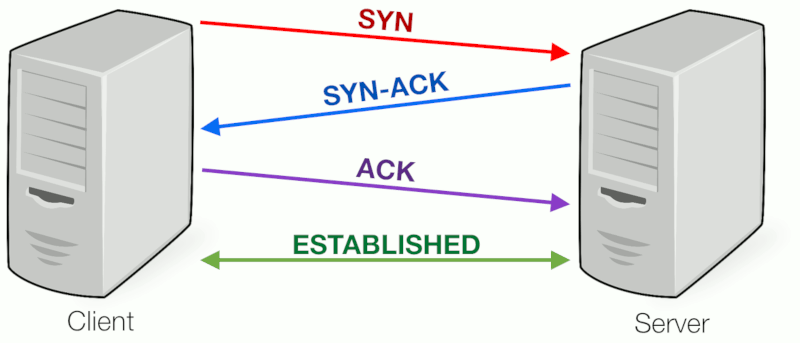
\includegraphics[width=0.7\linewidth]{figures/3-way-handshake}
	\caption{Graficzna reprezentacja uzgadniania trój-etapowego, https://www.luxoft-training.com/news/building-java-client-server-applications-with-tcp/}
	\label{fig:3-way-handshake}
\end{figure}

\emph{SYN Flood} polega na nadużyciu wyżej opisanej procedury. Atakujący przesyła do serwera falę komunikatów SYN, używając spreparowanych adresów IP. Niczego nieświadomy serwer odpowiada na żądania komunikatem SYN-ACK, po czym oczekuje na odpowiedź ACK od klienta celem sfinalizowania uzgodnienia trój-etapowego. Z racji faktu, iż serwer oczekuje na zakończenie komunikatu z fałszywymi adresami IP, połączenie to nigdy nie dojdzie do skutku. Efektem tego jest przeładowanie kolejki połączeń i ostatecznie pamięci operacyjnej serwera, powodując brak odpowiedzi na żądania zwykłych użytkowników. \cite{DDosHowItWorks}

Blokada danego adresu IP, z którego przychodzi wiele żądań w krótkim okresie czasu, nie stanowi większego problemu dla firewalli (zapór ogniowych), dlatego też coraz powszechniejszymi stają się ataki DDOS - \emph{Distributed Denial-Of-Service}. Różnica polega na tym, że żądania wysyłane są z wielu lokacji jednocześnie, co znacznie bardziej utrudnia identyfikację i zablokowanie nagłego ruchu przez zaporę ogniową.

Szybka detekcja nienaturalnego obciążenia serwera ma kluczowe znaczenie dla ochrony przed atakiem DDOS. W przypadku przedsiębiorstw wiąże się to także z zapewnieniem akceptowalnej jakości usług dla klientów oraz stratami, spowodowanymi niedostępnością serwisu. Istnieje wiele rozwiązań, które pozwalają wykrywać powyżej opisany incydent. Można je podzielić według sposobu ich działania i złożoności wykrywania. Do najskuteczniejszych rozwiązań należy analiza statystyczna ruchu, logika rozmyta, stosowanie sztucznych sieci neuronowych czy techniki eksploracji ukrytych zależności w repozytoriach danych. \cite{DDosDetection}

Ataki \emph{Denial of Service} stanowią zdecydowanie większe zagrożenie dla klasycznego modelu hostingu strony webowej, w którym celem zapewnienia dostępności serwisu korzysta się z fizycznych serwerów. W sytuacji, w której obciążenie aplikacji wzrośnie, przykładowo na skutek omawianego ataku, jedynym rozwiązaniem jest filtrowanie i odrzucanie potencjalnych złośliwych żądań - nie ma opcji na szybkie zwiększenie zasobów. 

W dzisiejszych czasach zdecydowanie lepszym rozwiązaniem zarówno pod kątem finansowym, jak i prostoty są publiczne chmury obliczeniowe, takie jak AWS (ang. Amazon Web Services), Microsoft Azure lub GCP (ang. Google Cloud Platform). Ich bogata oferta zapewnia podstawowe usługi takie jak dedykowane serwery, wirtualne sieci i interfejsy sieciowe czy usługi przechowywania danych. Ponadto chmury oferują usługi zaawansowanych mechanizmów przeciwdziałania atakom typu DDOS. Przykładem może być funkcjonalność chmury AWS w postaci grupy auto-skalującej (ang. auto-scaling group). Usługa ta dostosowuje liczbę instancji serwerowych w zależności od aktualnie panującego ruchu. Tak więc przy normalnych warunkach, gdy obciążenie serwera jest na niskim poziomie, w grupie może znajdować się jedna instancja serwerowa. Gdy tylko określony zasób przekroczy wcześniej zadeklarowaną wartość, na przykład zasoby procesora osiągną 80\% dostępnych zasobów w okresie minuty, automatycznie zostanie stworzona kolejna instancja serwerowa na podstawie pierwotnej. Tym samym ruch sieciowy zostanie rozłożony pomiędzy dwa serwery, zamiast jednego. 

Dobrym rozwiązaniem na tego typu ataki może być również użycie systemu równoważenia obciążenia - \emph{load balancera}. Jest to mechanizm, wykorzystywany w serwisach internetowych korzystających z większej ilości instancji serwerowych. W rezultacie każde połączenie jest przekierowane do jednego z dostępnych serwerów według następujących algorytmów:
\begin{itemize}
	\item \emph{Round Robin} - nadchodzące żądanie zostanie przekierowane do każdego serwera po kolei. Gdy dojdzie do końca, zrestartuje się.
	\item \emph{Least Connections} - \emph{Load Balancer} prześle żądanie do jednego z serwerów, które aktualnie procesują najmniejszą ilość żądań.
	\item \emph{IP Hash} - żądanie zostanie skierowane do najbliższego serwera pod kątem geolokalizacji. 
\end{itemize}

Ataki DOS są bezpośrednim zagrożeniem dla dostępności aplikacji webowych. Jeśli złośliwy ruch jest odpowiednio duży i nie zostanie szybko zidentyfikowany, może z łatwością przyczynić się do wyłączenia strony internetowej na nieokreślony czas. Dzięki wielu łatwo dostępnym narzędziom, takim jak systemy równoważenia obciążenia, grupy auto-skalujące, firewalle, ochrona przed tego typu zagrożeniem stała się dużo łatwiejsza niż kiedykolwiek.

...W kolejnej iteracji zawartość strony może zostać rozszerzona o dodatkowe elementy kursu, które pozwolą użytkowniki na "wirtualne" przeprowadzenie ataku, w którym będzie mógł zauważyć że strona która do tej pory działała, po uruchomieniu ataku jest niedostępna. 
\clearpage

\subsection{Phishing}
Phishing jest pewną formą socjotechniki, w której to atakujący, poprzez podszywanie się pod zaufane osoby lub instytucje, próbuje dokonać nieuczciwego przejęcia poufnych informacji od ofiary. Socjotechnika (inżynieria społeczna) to pewien zestaw sposobów wywierania wpływu na człowieka, aby ten dokonał czegoś wbrew swojej woli. Ataki phishingowe skierowane są zarówno do zwykłych użytkowników, jak i pracowników organizacji rządowych czy korporacji. Organizacja ulegająca atakowi może nie tylko ponieść poważne straty finansowe, ale również stracić reputację i zaufanie konsumentów. Badanie z 2021 r. firmy Kaspersky Lab, tworzącej popularne oprogramowanie antywirusowe Kaspersky wykazuje, że najpopularniejszymi organizacjami wykorzystywanymi przez phisherów są sklepy, portale internetowe i banki.  \cite{PhishingChart}	

\begin{figure}[H]
	\centering
	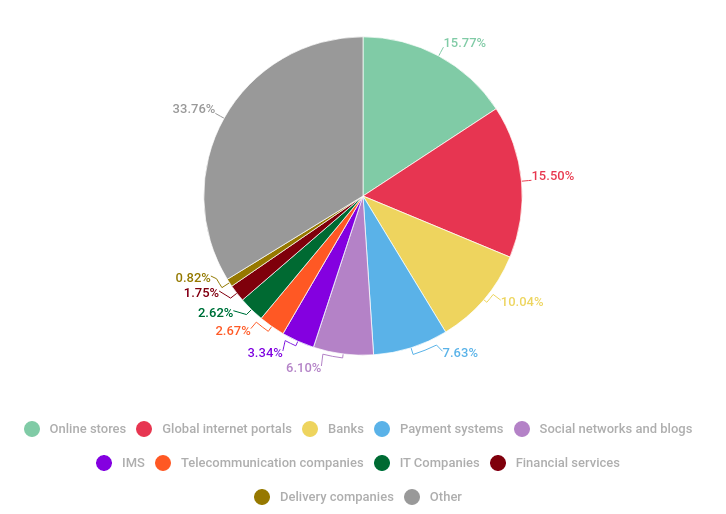
\includegraphics[width=0.9\linewidth]{figures/phishing-organisations}
	\caption{Ranking organizacji wykorzystywanych w atakach phishingowych, źródło: https://securelist.com/spam-and-phishing-in-q2-2021/103548/}
	\label{fig:phishing-organisations}
\end{figure}

Ataki przeprowadzone mogą być używając psychologicznej manipulacji wybranych osób celem uzyskania ich danych osobowych - forma inżynierii społecznej - albo przy użyciu dostępnych narzędzi informatycznych. Najczęściej występujące rodzaje phishingu to:

\begin{itemize}
	 \item E-maile phishingowe - spreparowana wiadomość phishingowa wysyłana jest na wiele skrzynek pocztowych, celem zwiększenia prawdopodobieństwa sukcesu ataku. Fałszywe wiadomości mogą zawierać cechy rzekomych organizacji, które miałyby być nadawcami, takie jak logo, stopkę, formatowanie celem skłonienia odbiorców do ujawnienia poufnych informacji, lub wejścia w złośliwe hiperłącze. \cite{PhishingEmails}
	 
	 \begin{figure}[H]
	 	\centering
	 	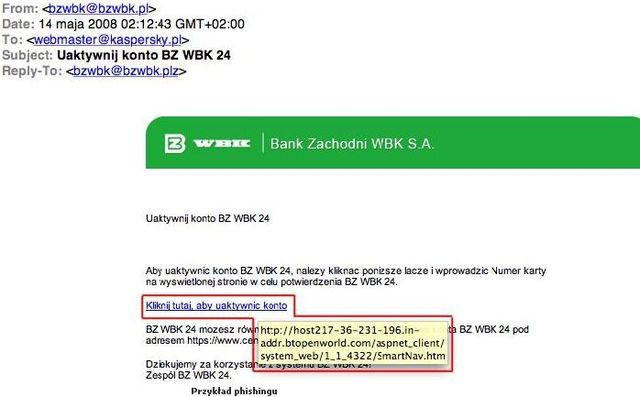
\includegraphics[width=1\linewidth]{figures/phishing-example}
	 	\caption{Przykład phishingu w formie wiadomości e-mail \cite{PhishingExample}}
	 	\label{fig:phishing-example}
	 	
	 \end{figure}
 
	 \item Fałszywa strona internetowa - polega na stworzeniu zwodniczo podobnej kopii strony internetowej poprzez tzw. \emph{Web Scrapping} \cite{WebScrapping} której celem jest przejęcie wrażliwych danych lub kradzież tożsamości użytkownika. Adres strony może być rozpowszechniany poprzez wiadomości SMS lub e-mail. \cite{WhatIsPhishing} 
	 
	 
	 \begin{figure}[H]
	 	\centering
	 	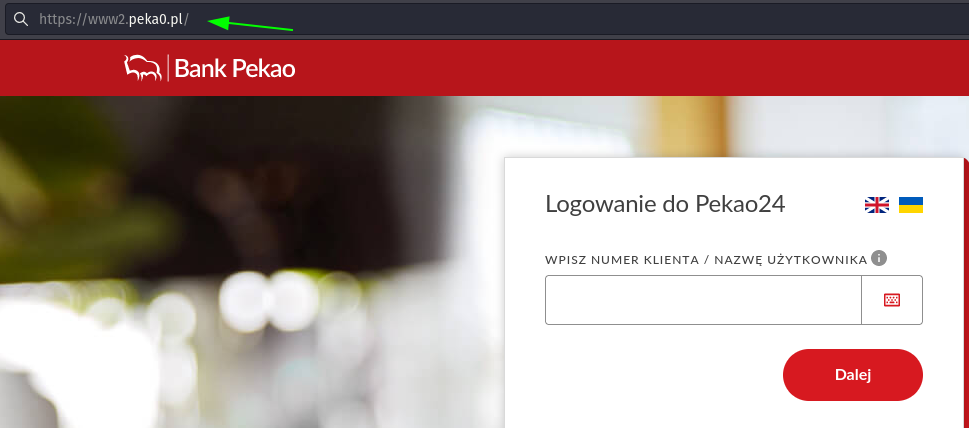
\includegraphics[width=0.96\linewidth]{figures/phishing-example2}
	 	\caption{Przykład phishingu w formie spreparowanej strony internetowej}
	 	\label{fig:phishing-example2}
	 \end{figure}
 
	 \item Phishing telefoniczny - przeprowadzany specyficznie za pomocą wiadomości SMS lub połączeń telefonicznych. Numery telefonów potencjalnych ofiar często pozyskiwane są w wyniku wycieków baz danych przedsiębiorstw lub organizacji. Atakujący kontaktując się z ofiarą, może podawać się za znaną jej osobę lub pracownika zaufanej instytucji, na przykład banku, celem zmanipulowania interlokutora do wykonania określonych akcji.
	 \item \emph{Pharming} - rodzaj phishingu, który jest znacznie trudniejszy w detekcji. Polega na zainfekowaniu serwera DNS lub urządzenia użytkownika w ten sposób, aby za każdym razem, gdy odwiedzana jest zaufana strona, nastąpiło przekierowanie na złośliwą, spreparowaną stronę internetową. 

\end{itemize}

Wektorami ataków phishingowych w większości przypadków są ludzie, a nie urządzenia. Szczególnie zagrożone są osoby niemające na co dzień styczności z internetem. Dobrym pomysłem jest - tam gdzie to możliwe - stosowanie uwierzytelniania wieloskładnikowego. Polega ono na potwierdzeniu próby autoryzacji poprzez dodatkowy element: kod wysyłany wiadomością SMS lub e-mail. Zapobiega to sytuacjom, w których to dane autoryzacyjne poszkodowanego takie jak adres e-mail i login zostaną użyte przez niewłaściwe osoby. Nie będą one mogły w pełni się uwierzytelnić, jeśli nie posiadają kodu autoryzacyjnego. Dodatkowo może stanowić ostrzeżenie dla ofiary, że ktoś próbuje zalogować się na jej konto. Zaufanym rozwiązaniem są również programy antywirusowe, ostrzegające użytkownika przed fałszywymi domenami oraz odpowiednio skonfigurowane filtry anty-spamowe w poczcie e-mail.

Należy także uważnie sprawdzać adresy URL stron internetowych, na których podaje się wrażliwe dane. Phisherzy często wykorzystują podobieństwo niektórych cyfr i liter, na przykład ``0'' i ``o'' celem stworzenia złudzenia, że użytkownik znajduje się na właściwej stronie. Istotnym elementem jest również protokół, który użyty został do połączenia ze stroną. Zdecydowana większość organizacji korzysta z ważnych certyfikatów SSL, sprawiając, że połączenie między klientem a serwerem jest szyfrowane (HTTPS).

\clearpage
\subsection{Ransomware}
\emph{Ransomware} to typ złośliwego oprogramowania (ang. malware), którego celem jest zablokowanie dostępu do komputera osobistego poprzez zaszyfrowanie wszystkich możliwych plików. Czas trwania tej procedury zależy między innymi od wybranego algorytmu szyfrowania i danych na szyfrowanym urządzeniu, jednak w przypadku zwykłego użytkownika domowego może wykonać się w czasie zaledwie dwóch godzin \cite{RansomwareTime}. Zazwyczaj ten czas jest znacznie dłuższy, gdyż przed rozpoczęciem procesu wymagany jest dokładny rekonesans systemu i struktury katalogów. Tym sposobem użytkownik traci możliwość odczytu danych na swoim urządzeniu, a do odszyfrowania plików, wymagany jest klucz posiadany przez atakującego. 

Ten rodzaj szkodliwego oprogramowania jest szczególnie niebezpieczny dla przedsiębiorstw, gdyż utrata ważnych dokumentów czy danych finansowych, może się wiązać z poważnymi konsekwencjami, lub brakiem możliwości reakcji na czas (np. złożeniu oferty w terminie). Celem \emph{ransomware} nie jest usunięcie lub kradzież plików, ale zablokowane ich, i oczekiwanie na ewentualną zapłatę okupu przez ofiarę. 

Sposoby, poprzez które złośliwe oprogramowanie dostaje się do przedsiębiorstw, przedstawione są na poniższym rysunku, przygotowanym przez organizację CoveWare \cite{RansomwareAttackVectors}, specjalizującą się w przeciwdziałaniu rozprzestrzeniania się tego typu atakom:
\begin{figure}[ht]
	\centering
	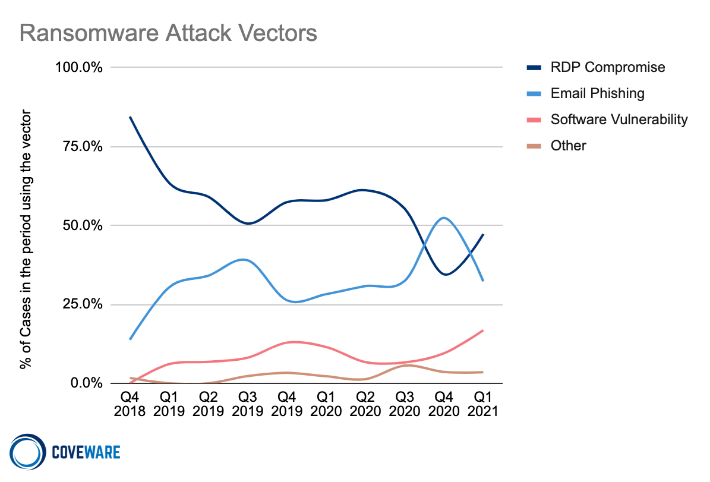
\includegraphics[width=13cm]{figures/ransomware-attack-vectors.png}
	\caption{Wektory ataku ransomware}
	\label{Fig:Wektory ataku ransomware}
\end{figure} 

Jak można zauważyć, obecnie wiodącym źródłem dystrybucji tego złośliwego oprogramowania jest Remote Desktop Protocol (RDP) \cite{RDP} - protokół umożliwiający połączenie się z maszyną z systemem MS Windows, oraz przejęcie nad nim pełnej kontroli, używany w firmach jako narzędzie do konfiguracji urządzeń. 

Kolejno znajdują się e-maile phishingowe, opisane w poprzednim rozdziale. Ten sposób zazwyczaj polega na odpowiednim wykorzystaniu inżynierii społecznej, celem zmanipulowania ofiary do udzielenia poufnych danych dostępowych lub uruchomienia oprogramowania szyfrującego na swoim urządzeniu.  

Istotną regułą, którą należy się kierować przeciw tego typu złośliwemu oprogramowaniu w przedsiębiorstwie jest Zasada najmniejszego uprzywilejowania (ang. Principle of least privilege). Polega ona na zapewnieniu dostępu ... tylko do tych zasobów do których jest to konieczne przy wykonywaniu standardowych działań. Ogranicza to dostęp do wrażliwych ... do minimum, co znacznie utrudnia infekcję najbardziej krytycznych elementów infrastruktury takich jak serwery produkcyjne, [miejsca do przechowywania wrazliwych danych, backupow itp]. Opisac tez Zasade Ograniczonego zaufania

Najlepszą metodą przeciwko tego  jest systematyczne wykonywanie archiwizacji danych. W sytuacji w której \emph{ransomware} trafi do komputera i zaszyfruje wszystkie pliki, pozostaje jedynie odtworzyć kopię zapasową. Dobrym sposobem jest także częste aktualizowanie systemu operacyjnego, celem eliminowania potencjalnych luk bezpieczeństwa.

\clearpage


\subsection{Podatność XSS}

\emph{Cross-site scripting} (XSS) jest jedną z najbardziej niebezpiecznych podatności zagrażających współczesnym aplikacjom webowym. XSS jest atakiem skierowanym na klienta korzystającego serwisu webowego, w przeciwieństwie do np. \emph{SQL Injection}, którego celem jest aplikacja działająca po stronie serwera. \emph{Cross-site scripting} opiera się głównie na wstrzyknięciu do strony internetowej złośliwego skryptu, który, dla przykładu, może odczytać ciasteczka użytkownika lub inne poufne informacje, które przechowuje przeglądarka, wysłać je do atakującego, aby ten -- używając zapisanych w ciasteczkach danych -- mógł zalogować się na konto użytkownika, który nieświadomie uruchomił dany skrypt. Poprzez ten atak, można również uruchomić Keyloggera (narzędzie do przechwytywania aktywności klawiatury) działającego w przeglądarce, lub całkowicie zmienić zawartość strony internetowej. 

W raporcie przygotowanym w 2017 roku przez Wordfence, komercyjną organizację zajmującą się zabezpieczaniem stron internetowych przed wszelkimi niebezpieczeństwami, wynika, iż ten typ podatności stanowi blisko połowę wszystkich podatności w sieci. \cite{XSSReport}

\begin{figure}[H]
	\centering
	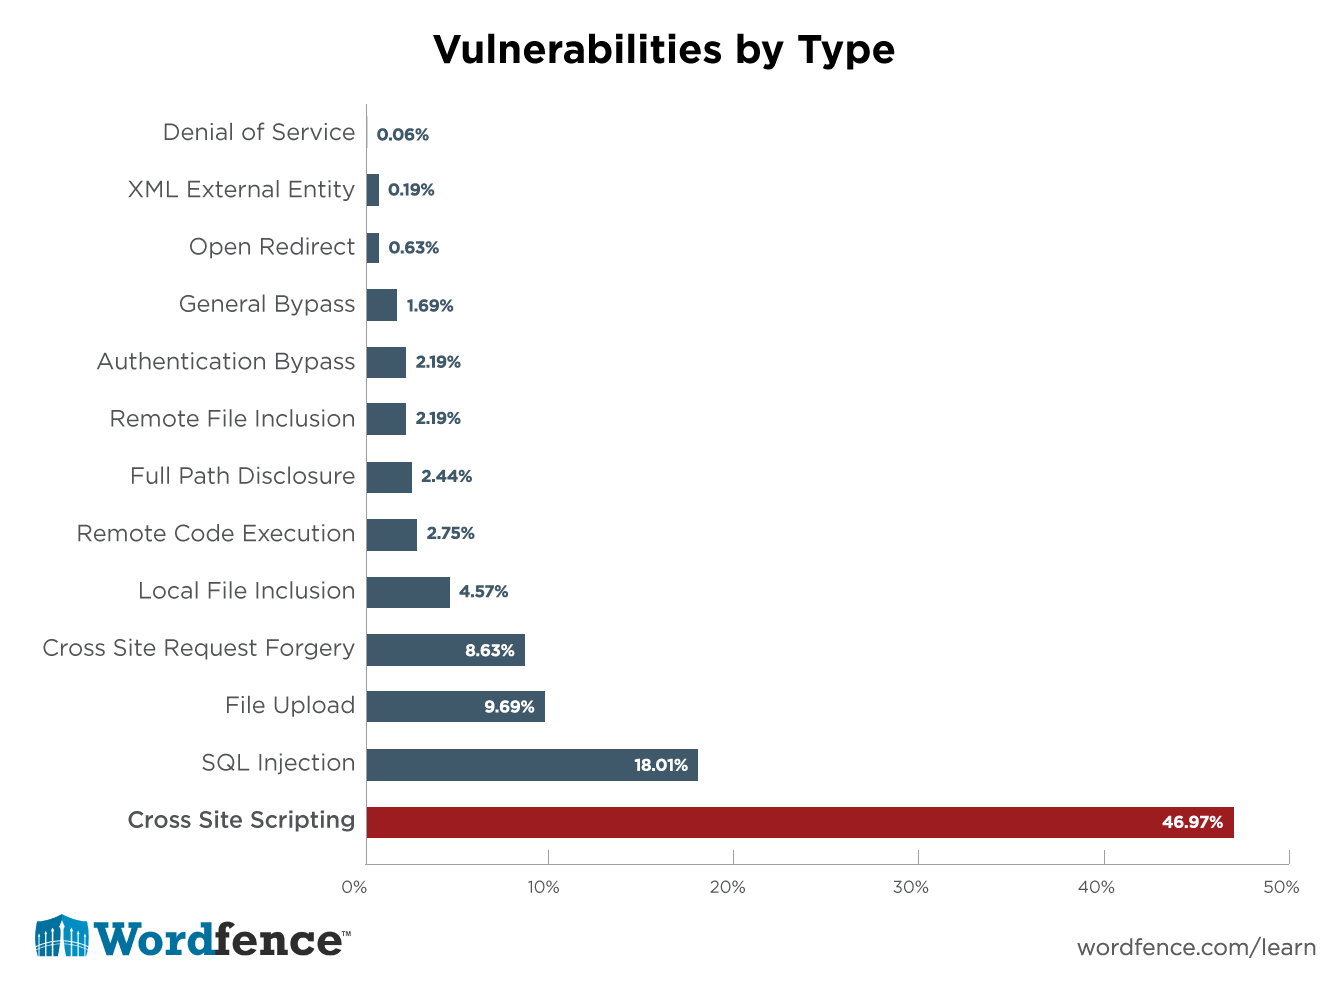
\includegraphics[width=0.9\linewidth]{figures/xss-popularity}
	\caption{Klasyfikacja podatności aplikacji internetowych pod kątem częstotliwości występowania}
	\label{fig:xss-popularity}
\end{figure}



Opisując XSS nie sposób nie wspomnieć o Regule Tego Samego Pochodzenia (\emph{Same-Origin Policy}) \cite{SameOriginPolicy}. Jest to jeden z wielu fundamentalnych mechanizmów bezpieczeństwa, zaimplementowany w każdej przeglądarce internetowej. Nie pozwala on żadnej stronie na podjęcie akcji lub odczytania zawartości innej strony, na przykład w dwóch kartach przeglądarki. W związku z tym, wszystko, co się dzieje na stronie internetowej otwartej przez użytkownika, jest izolowane i nie będzie miało wpływu na pozostałe otwarte strony.

[FORMAT] Tworem powiązanym z {\emph{Same-Origin Policy} są narzędzia pozwalające na sandboxing...

Cała struktura strony internetowej zakodowana językiem HTML może być zmieniana poprzez JavaScript, używając DOM API \cite{DOM}. Jako rezultat, prosty skrypt może całkowicie zmienić zawartość, wygląd, a przede wszystkim funkcjonalność strony internetowej.

Ciasteczkami (ang. cookies) \cite{Cookies} nazywa się niewielkie porcje informacji wysyłane przez serwer do przeglądarki internetowej urządzenia końcowego. Służą do tego, by zapisać obiekty danych w plikach przeglądarki, które przy ponownym odwiedzeniu strony, mogą być przesłane do tego samego serwera, z którego przyszły. W związku z tym, przy odwiedzaniu różnorakich stron wymagających autoryzacji, użytkownik nie musi się za każdym razem logować, gdyż wszystkie potrzebne dane są zawarte w ciasteczkach, które przesyłane są razem z żądaniem. 

Ataki XSS można podzielić na trzy główne kategorie:

\begin{itemize}
	\item \emph{Reflected XSS} - złośliwy skrypt umieszczony jest w adresie URL. Po wejściu w hiperłącze, ofiara nieświadomie wykonuje wcześniej przygotowany skrypt, rezultatem czego jest wykonanie kodu w przeglądarce.
	\item \emph{Stored XSS} - polega na umieszczeniu skryptu po stronie serwera, przykładowo jako wiadomość w serwisie społecznościowym. Po odczytaniu jej przez ofiarę, automatycznie wykonywany jest wcześniej przygotowany skrypt, co może skutkować wysłaniem ciasteczka sesyjnego innego użytkownika do atakującego, pozwalając mu na umieszczenie skradzionego ciasteczka w przeglądarce i nieautoryzowany dostęp do konta ofiary.
	\item \emph{DOM Based XSS} - atak ściśle powiązany z modyfikacją struktury DOM. Sama odpowiedź HTTP nie ulega zmianie, jednak kod po stronie klienta zawarty w aplikacji wykonywany jest w inny sposób z powodu modyfikacji, które miały miejsce w DOM.
\end{itemize}

Najczęstszym miejscem, w którym można spotkać tę podatność, są formularze, do których użytkownik wpisuje treść, która następnie jest wyświetlana. Jeśli treść którą przesłał użytkownik nie zostanie odpowiednio wyczyszczona, może dojść do sytuacji, w której to użytkownik wstrzyknie złośliwy skrypt.

[FORMAT WYJASNIC O CO CHODZI]

Przeglądarki internetowe zostały wyposażone wiele narzędzi do walki z tą podatnością, takich jak system wykrywania złośliwego kodu JavaScript. Mechanizm ten składa się z wbudowanego w przeglądarkę komponentu analizy skryptów oraz systemu IDS (ang. Intrusion Detection System), przetwarzającego aktywność po stronie klienta, i porównującego ją ze znanymi złośliwymi skryptami. Dzięki temu systemowi możliwe jest wykrywanie różnego rodzaju ataków XSS. Jednak system ma znaczną wadę: może wykryć tylko sytuacje, których zachowanie jest mu znane -- nie jest odporny na nowe typy ataku. \cite{XSSProtection}

Pomimo wielu zabezpieczeń, które są wbudowane w przeglądarki, te nie są w stanie odróżnić czy dany skrypt jest złośliwy, czy nie - dlatego też odporność aplikacji internetowej na tego typu atak stoi przede wszystkim po stronie programistów.

Najskuteczniejszą ochroną przed atakami XSS jest filtrowanie danych przychodzących od użytkownika przed tym, kiedy to mają zostać wyświetlone w aplikacji, na przykład poprzez zamianę znaków tagów HTML na znaki specjalne \cite{XSSSpecialTags}. Skutecznym rozwiązaniem może być także oczyszczanie wprowadzonej treści użytkownika z elementów wspólnych dla każdego ataku XSS, na przykład tagów <script></script>.

TODO - dopisac jeszcze jak sie bronic, i dodac przyklad na podstawie kodu i przegladarki
\clearpage

\subsection{Keylogger}

Keyloggery występują zazwyczaj w formie złośliwego, ukrytego oprogramowania. Nie są widoczne na pierwszy rzut oka dla użytkownika i w zdecydowanej większości przypadków działają w tle, często podszywając się pod inną aplikację, tym samym maskując swoją obecność. 

Podstawowe właściwości tego typu programu można opisać jako przejmowanie kontroli nad procedurami związanymi z obsługą klawiatury systemu operacyjnego, na którym się znajduje.

Głównym celem tego oprogramowania jest zbieranie danych o tym, jakie klawisze na klawiaturze zostały naciśnięte przez użytkownika w jakiej kolejności, a następnie okresowe wysyłanie zebranych informacji do atakującego. Posiadając wiedzę na temat tego, co zostało wpisane na urządzeniu, można bez problemu uzyskać dostęp do wrażliwych informacji takich jak prywatna korespondencja, poufne dane czy hasła. Do bardziej zaawansowanych funkcji należy między innymi przesyłanie zrzutów ekranu, rejestrowanie historii otwieranych programów i przekazywanie tych informacji dalej.

Keyloggery oprócz formy programowej istnieją również jako osobne urządzenia, które podłączane są do jednostki zazwyczaj poprzez interfejs USB. Mogą także występować jako urządzenie pośredniczące pomiędzy klawiaturą a złączem USB komputera. 

Sposobem na unikanie tego typu oprogramowania jest przede wszystkim systematyczne sprawdzanie uruchomionych procesów, ale także używanie odpowiedniego antywirusa.
\clearpage

\subsection{CSRF}
Cross Site Request Forgery (CSRF) jest atakiem na aplikacje internetowe, którego celem jest wykonanie przez użytkownika końcowego niechcianej akcji w serwisie w którym aktualnie jest on zalogowany. 
[FORMAT ROZBIC WYZEJ NA DWA]


Ten typ ataku jest wykorzystywany szczególnie gdy oprogramowanie serwisu internetowego nie jest wykonane zgodnie ze standardami bezpieczeństwa OWASP (ang. Open Web Application Security Project). \cite{OWASP10}.

Warunkiem koniecznym na wystąpienie tej podatności jest aktywna sesja użytkownika w danej witrynie webowej oraz aktywny token autoryzacyjny (uzyskiwany zazwyczaj jako odpowiedź serwera na poprawne dane użytkownika przy mechanizmie logowania na stronie internetowej). Następnie przechowywany jest on w pamięci przeglądarki przez wybrany okres czasu.

Spreparowane żądanie może być stworzone na wiele sposobów. Dla przykładu, w sytuacji w której klient banku chce wykonać przelew bankowy, utworzone żądanie w podatnej, błędnie wykonanej aplikacji będzie miało następującą formę:

\

\begin{lstlisting}[caption=Przykładowe żądanie aplikacji podatnej na CSRF,label={KodPHP1}]
	GET https://bank.com/transfer?amount=100&accountNumber=123456 HTTP/1.1. 
\end{lstlisting}

Jeśli dojdzie do sytuacji że w przeglądarce będzie znajdywał się token autoryzacyjny zapisany w ciasteczkach lub pamięci lokalnej, ofiara po wejściu  w hiperłącze \
{https://bank.com/transfer?amount=100\&accountNumber=123} nieświadomie wykona to żądanie, co będzie skutkowało przelaniem określonej kwoty pieniędzy na wybrane konto przez atakującego. Link ten może zostać dostarczony poprzez stosowanie odpowiednich środków psychologicznych i metod manipulacji (inżynierię społeczną) lub maile phishingowe. Aplikacja nie jest w stanie odróżnić czy żądanie od klienta końcowego przyszło zgodne z jego intencjami, czy też nie. 

W dzisiejszych czasach, zdecydowana większość szkieletów do tworzenia aplikacji webowych posiada mechanizmy zabezpieczające budowaną stronę przed tą podatnością. Jeśli jednak wybrana technologia nie posiada wbudowanego mechanizmu, koniecznym będzie dodanie tokenów CSRF do wszystkich żądań wpływających na stan aplikacji. Z każdym żądaniem do serwera powinien być wysyłany jednorazowy token - ciąg losowych znaków, a następnie powinien być on walidowany wraz z wszystkimi danymi które znajdują się w ciele lub parametrach żądania. 


\clearpage

\section{Podsumowanie i wnioski końcowe}

...W dzisiejszych czasach jest to bardzo poszukiwane

...jesli ktos nadal uwaza ze kwestie cyberbezpieczeństwa sa poboczne, marginalne lub obecnie stanowia jedynie mniej istotna czesc szeroko rozumianej teleinformatyki a skutki nie maja tak znaczacego wplywu na indywidualne osoby powinien zwrocic uwage na niedawna luke typu 0day w postaci log4j pokazalo jak to jest biezacy temat

...moge zacytowac https://edukomiks.pl/, jest to tematyka powszechna cyberbezpieczestwa, czego dowodem jest to ze powstaja takie rzeczy nawet dla rzeczy, dotykam seizego problemu w swojej pracy ze mozna sobie tego poradzic

...W procesie programowania strony internetowej i tworzenia treści kursów wiele się nauczyłem, pogłębiłem wiedzę, poznałem klasyfikacje i systematyke wiem w kakich obszarach dane zagrozenie wystepuje i uwazam ze stworzyl wartosciowy material szkoleniowy ktory moze zostac wykrozystany komercyjnie. nie bylo wiele wykladow kursowych wiec ueazam ze wykonalem wiele rpacy poprzez studia literatury i prac praktyczntch w i ter ecie dotyczacych zagrozen w it, to ze przebilem sie przez ten trmat to byl wynik moj
\clearpage

\addcontentsline{toc}{section}{Literatura}

@TODO - posegregowac, naprawic opisy itemow

\begin{thebibliography}{4}
	
\bibitem{sekurak} M. Bentkowski, G. Coldwind , A. Czyż, R. Janicki, J. Kamiński, A. Michalczyk, M. Niezabitowski, M. Piosek, M. Sajdak, G. Trawiński, B. Widła. Bezpieczeństwo aplikacji webowych
\bibitem{JS} https://developer.mozilla.org/en-US/docs/Learn/JavaScript/First{\_}steps/What{\_}is{\_}JavaScript. Dostęp 11.06.2021.
\bibitem{SameOriginPolicy} https://developer.mozilla.org/en-US/docs/Web/Security/Same-origin{\_}policy. Dostęp 12.06.2021.
\bibitem{DOM} https://developer.mozilla.org/en-US/docs/Web/API/Document{\_}Object{\_}Model. Dostęp 12.06.2021. 
\bibitem{Cookies} https://developer.mozilla.org/en-US/docs/Web/HTTP/Cookies. Dostęp 12.06.2021.
\bibitem{RDP} https://docs.microsoft.com/en-us/troubleshoot/windows-server/remote/understanding-remote-desktop-protocol. Dostęp 02.08.2021.
\bibitem{RansomwareAttackVectors} https://www.coveware.com/blog/ransomware-attack-vectors-shift-as-new-software-vulnerability-exploits-abound. Dostęp 02.08.2021.
\bibitem{RansomwareTime} https://thedfirreport.com/2020/10/18/ryuk-in-5-hours. Dostęp 03.08.2021.
\bibitem{Ddos} https://www.cloudflare.com/learning/ddos/what-is-a-ddos-attack. Dostęp 24.06.2021.
\bibitem{Nodejs} https://www.educative.io/blog/what-is-nodejs. Dostęp 03.08.2021.
\bibitem{OWASP10} https://owasp.org/www-project-top-ten. Dostęp 10.07.2021.
\bibitem{WhatIsPhishing} Tom N Jagatic, Nathaniel A Johnson, Markus Jakobsson, Filippo Menczer, Social phishing (2007/10/1)
\bibitem{PhishingChart} https://securelist.com/spam-and-phishing-in-q1-2021/102018. Dostęp 02.09.2021.
\bibitem{PhishingEmails} Phishing Attacks: A Recent Comprehensive Study and a New Anatomy, Chaminda Hewage, Liqaa Nawaf, Imtiaz Ali Khan, Zainab Alkhalil
\bibitem{BigData} Raport ITwiz: Internet Rzeczy i Big Data w praktyce
\bibitem{JavascriptPopularity} Amantia Pano Daniel Graziotin Pekka Abrahamsson, Factors and actors leading to the adoption of a JavaScript framework 
\bibitem{DDosHowItWorks} DoS and DDoS Attacks: Impact, Analysis and Countermeasures, Nikhil Tripathi, Babu Mehtre
\bibitem{3WayHandshake} https://www.sciencedirect.com/topics/computer-science/three-way-handshake. Dostęp 19.09.2021.
\bibitem{DDosDetection} A novel approach for mitigating the effects of the TCP SYN flood DDoS attacks, Mitko Bogdanowski, Aleksandar Toshevski, Marjan Bogdanoski, Dimitar Bogatinov
\bibitem{XSSProtection} Prevention Of Cross-Site Scripting Attacks (XSS) On Web Applications In The Client Side, S.Shalini, S.Usha
\bibitem{XSSReport} https://www.wordfence.com/learn/how-to-prevent-cross-site-scripting-attacks. Dostęp 28.09.2021.
\bibitem{XSSSpecialTags} https://dev.w3.org/html5/html-author/charref. Dostęp 28.09.2021.
\bibitem{NodejsWhatIs} Using Node.Js to Build High Speed and Scalable Backend Database Server, S. L. Bangare, S. Gupta, M. Dalal, A. Inamdar
\bibitem{WebScrapping} https://www.imperva.com/learn/application-security/web-scraping-attack. Dostęp 29.09.2021.
\bibitem{PhishingExample} https://www.egospodarka.pl/art/galeria/39266,Bankowosc-online-a-zabezpieczenia,1,12,1.html. Dostęp 01.10.2021.
\bibitem{VrLearning}
Virtual Reality in the Learning Process, Bayron Chavez, Sussy Bayona
\bibitem{Deepl}
https://www.deepl.com/en/blog/how-does-deepl-work. Dostęp 30.01.2022
\bibitem{ReactPopular} Most popular web frameworks among developers worldwide 2021, Shanhong Liu, 15.12.2021
\end{thebibliography}

\clearpage

\makesummary

\end{document} 
